\chapter{Improving Build Times}
The project groups want the build times on Jenkins to be faster. When multiple changes are pushed to the master branch within a short space of time, they will create congestion the build queue. This means that even though the build itself may take only a few minutes, the time it takes from push to finished build may be much longer (and exceed than the 10 minutes advocated by Kent Beck \parencite{beck2004}).

We measure the time different parts of the Launcher project take to identify in which parts of the build process to make faster. The Launcher project is the main application which depends on many other subprojects (henceforth a ``dependency''). These dependencies are managed as Git submodules \parencite{git-submodules-doc}, which basically clones the contents of a repository (the dependency) at a specific revision into another repository (the dependent project). The build timings are measured on the Jenkins server and shown in \figureref{fig:launcher_build_times_1}. The shows the build timings of the Launcher application and the different dependencies (\emph{Oasis-lib, Giraf-Component, Local-db, Barcode-scanner, and Metadata}), as well as the startup time for the emulator. As can be seen, the emulator and the Giraf-component and Oasis-lib projects have the most significant influence on build times. These three parts use about \SI{90}{\percent} of the total build time. The actual Laucher application itself takes only very little part of the total build time.

To understand which parts of the dependencies that take time, we measure the individual build steps (tasks) performed during a build. These can be seen in \appendixref{app:build_times}. The reason that the Oasis-lib dependency takes a long time to build is that it contains a great number of tests which run on the emulator. These tests are run every time a project depending on Oasis-lib builds --- even though the library itself has not been updated. The most significant task when building the Giraf-Component library is the test task as well. However, the Giraf-Component library only contains one simple test, so we do not expect the actual test execution time to use much of this time. Instead, we expect it to be caused by the order in which projects are tested. When preparing the tests, the tests from all projects are combined into a single Android application package (APK-file). The first test task run is responsible for installing this application on the emulator, while the subsequent test tasks can skip this step. Because the Giraf-components project is the first in the sequence of libraries to be tested, this task also installs the tests on the emulator which is likely to take some time.
\todo{Overvej flere målinger og tag gennemsnit}
\begin{figure}
  \centering
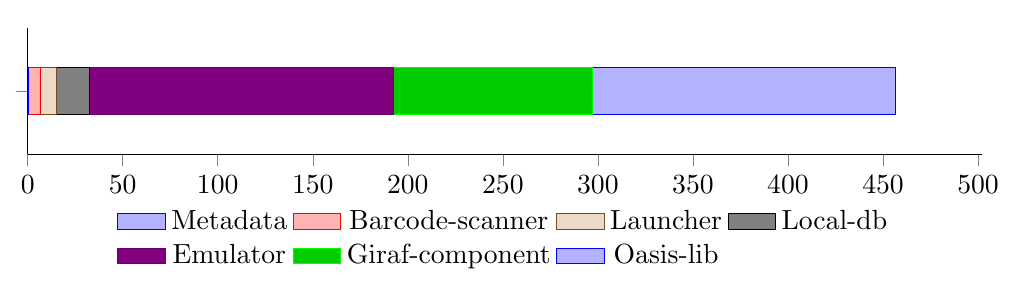
\begin{tikzpicture}[trim axis left, trim axis right]
  \begin{axis}[
    xbar stacked,
    scale only axis,
    width=\textwidth,
    axis y line*= none, axis x line*= bottom,
    %xmajorgrids = true,
    ytick = data,
    yticklabels = {},
    tick align = outside,
    %xtick pos = left,
    bar width=6mm,
    y=8mm,
    %nodes near coords,
    legend style={
      at={(0.5,-0.35)},
      legend columns=4,
      anchor=north,
      yshift=0ex,
      xshift=0ex,
      draw=none
      %legend cell align=left
    },
    area legend,
    xlabel = {Time (seconds)},
    xmin = 0
  ]
    \addplot coordinates
    {(0.2,0)};
    \addlegendentry{Metadata}
    \addplot coordinates
    {(6.625,0)};
    \addlegendentry{Barcode-scanner}
    \addplot coordinates
    {(8.393,0)};
    \addlegendentry{Launcher}
    \addplot coordinates
    {(17.223,0)};
    \addlegendentry{Local-db}
    \addplot coordinates
    {(160.000,0)};
    \addlegendentry{Emulator}
    \addplot coordinates
    {(104.696,0)};
    \addlegendentry{Giraf-component}
    \addplot coordinates
    {(159.497,0)};
    \addlegendentry{Oasis-lib}
    %\legend{Test, test, test, test, test, test}
  \end{axis}
\end{tikzpicture}
\caption{Timings during build of the Launcher project before updating emulator plugin.}\label{fig:launcher_build_times_1}
\end{figure}

To improve the overall build times, we look at how to speed up the emulator and to avoid running tests on the dependencies every time a project is build. We first update the Android Emulator Jenkins plugin to a new version with improved emulator stability. We do this to ensure that we do not work on improving parts which are already improved in the most recent version of the plugin. After updating, we measure the build times again. As shown in \figureref{fig:launcher_build_times_2}, the emulator startup time is significantly increased. Because of this, the emulator startup time is no longer the primary concern, and we focus on decreasing the dependency build times. \todo{Vi kan måske beskrive test uden emulator her, og konkludere at det ikke er arbejdet værd}

\begin{figure}
\centering
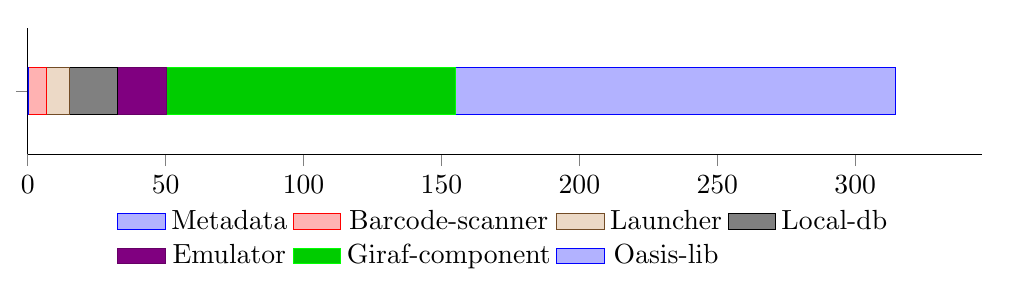
\begin{tikzpicture}[trim axis left, trim axis right]
  \begin{axis}[
    xbar stacked,
    scale only axis,
    width=\textwidth,
    axis y line*= none, axis x line*= bottom,
    %xmajorgrids = true,
    ytick = data,
    yticklabels = {},
    tick align = outside,
    %xtick pos = left,
    bar width=6mm,
    y=8mm,
    %nodes near coords,
    legend style={
      at={(0.5,-0.35)},
      legend columns=4,
      anchor=north,
      yshift=0ex,
      xshift=0ex,
      draw=none
      %legend cell align=left
    },
    area legend,
    xlabel = {Time (seconds)},
    xmin = 0
  ]
    \addplot coordinates
    {(0.209,0)};
    \addlegendentry{Metadata}
    \addplot coordinates
    {(6.625,0)};
    \addlegendentry{Barcode-scanner}
    \addplot coordinates
    {(8.393,0)};
    \addlegendentry{Launcher}
    \addplot coordinates
    {(17.223,0)};
    \addlegendentry{Local-db}
    \addplot coordinates
    {(18.000,0)};
    \addlegendentry{Emulator}
    \addplot coordinates
    {(104.696,0)};
    \addlegendentry{Giraf-component}
    \addplot coordinates
    {(159.497,0)};
    \addlegendentry{Oasis-lib}
    %\legend{Test, test, test, test, test, test}
  \end{axis}
\end{tikzpicture}
\caption{Timings during build of the Launcher project.}\label{fig:launcher_build_times_2}
\end{figure}

One obvious way of decreasing overall build times is to use faster hardware on the server. However, because the multi-project has no financial income, buying new hardware is generally the last resort. In addition, it is difficult to estimate exactly how much of an decrease this will give in practice. Another option is to not test dependencies when dependend projects are build, but only when changes happen in the actual dependency project. While this will decrease the overall build times, each dependency is still built every time a dependend project is built, which limits the amount by which we can decrease the total build times. There may as well arise some quality assurance issues by not testing each build of the dependency. Because of this, we look at improving the build times in a different way, specifically by using pre-compiled libraries.

\section{Dependency Management}
Instead of building and testing dependencies each time a dependend project is built, we look at referring pre-compiled and pre-tested library files. We are inspired by the way \mono{.\@jar}-files are typically used as libraries for Java projects. This way of managing libraries has a number of advantages compared to the current setup:
\begin{description}
  \item [Pre-Compiled and Pre-Tested] Libraries are binary pre-compiled and pre-tested files. This means that dependend projects do not have to build ant test all depencencies, which decreases the build time significantly.
  \item[Quality Control] Libraries are built and released only if the tests pass, so there will never be dependencies which cannot compile or do not work\footnote{Of course, there may be bugs even if all tests pass, but the risk is decreased}.
  \item[Cleaner Structure] Nested dependencies (dependency A depends on dependency B which depends on dependency C) is well defined and nicely handled. The individual libraries do not include their dependencies, so it is always the dependend library that has to include all dependencies. Currently, the same dependency may be included multiple times in the same project.
\end{description}
The Android counterpart of Java \mono{.\@jar}-files are \mono{.\@aar}-files. These files are similar to \mono{.\@jar}-files, except that they can contain Android-specific dependencies such as icon resources as well \parencite{android-aar}.

With this solution, it is clear that we no longer want to use submodules for managing dependencies. Coincidentally, the Git-responsible group in the multi-project work on a user story which states ``Remove Git submodules''. The reason for this user story is that the developers generally find the submodules difficult to work with. Because this overlap with our solution to making build times faster, we decide to solve this in collaboration.

\subsection{Agreement Upon Submodule Replacement}
The Git-responsible group initially propose to remove submodules by merging all repositories into one, each project having its own directory located in the root directory of the repository, as shown in \figureref{fig:single_repo_structure}. Dependencies are then handled by referring to the relative path of the dependency. For example, if \mono{ProjectA} depends on \mono{ProjectB}, \mono{ProjectA} will contain a reference to \mono{../ProjectB}.
\begin{figure}
  \dirtree{%
.1 /.
.2 ProjectA.
.3 \ldots.
.2 ProjectB.
.3 \ldots.
.2 ProjectC.
.3 \ldots.
.2 ProjectD.
.3 \ldots.
}
\caption{Single repository file structure} \label{fig:single_repo_structure}
\end{figure}

\todo{Beskriv ulemperne ved denne løsning}
% Husk at skrive om trace-back
% Se \parencite{fowlerReproducibleBuild}
% http://martinfowler.com/bliki/ReproducibleBuild.html

\subsection{Dependency Repository}
\todo{Skriv hvorfor versionskontrol er vigtigt}
\todo{Skriv hvorfor vi skal have et repository}
% http://www.oracle.com/technetwork/articles/java/enterprise-binaries-2227134.html
% http://blogs.collab.net/subversion/why-you-should-be-using-an-artifact-repository-part-1#.VSEWcpOsUkM